%2011.4.4 ヤマサキ この章は大きく変更した箇所はありません。
\chapter{慣性系と慣性力}

車がカーブする時に搭乗者は回転の外側にひっぱられる力を
感じる。エレベーターに乗ると, エレベーターが動き始めたり止まったり
するときに身体が重くなったり軽くなったり感じる。このような力を
慣性力という。慣性力は, 地球の気象現象を司る「コリオリ力」
の源であり, また, 農業機械の自動運転に欠かせない「慣性計測装置」
の原理でもある。この章では, 慣性力について学ぼう。


\section{慣性系と慣性の法則}
質点の位置$(x, y, z)$とは, どこかにある「原点」$(0, 0, 0)$
と, どちらかに向かう座標軸($x$軸, $y$軸, $z$軸)の組み合わせ, つまり座標系を
定めることによって初めて定量的に定まる概念だ。
つまり, 座標系が無ければ位置は定まらない。位置の(時刻による)微分が速度であり, 
速度の(時刻による)微分が加速度なのだから, 位置が定まらなければ速度も加速度も
定まらない。加速度が定まらねば運動方程式は意味を持たない。すなわち, 座標系が
無ければ運動の法則も無いのだ。

では, 「座標系」というのは, どのようにして与えられるのだろうか? たとえばつくば市の
どこかの地点を「原点」と定めて, そこから東西南北と上下に座標軸を張れば, それはひとつの
座標系だが, それ以外にも座標系はあり得る。ハワイやフランクフルトあたりに
原点を置くこともできるだろう。あるいはつくばエクスプレスの, 走行中の快速電車の
先頭車両の真ん中に原点を定めて, 進行方向に$x$軸, 右方向に$y$軸, などと定めること
もできるだろう。そんなのありか!?と思うかもしれないが, 座標系は静止していなくても
よいのだ。そもそも「静止」という考え方が, 何か特定の座標系を基準に
したときにのみ成り立つ概念であり, どれかの座標系で見れば静止している質点も, 
別の座標系で見れば動いている, ということは十分にありえるのだ。

そういうわけで, 座標系の与え方には任意性があるし, 座標系の与え方によって運動の
様子も違って見える。実は, 我々がこれまで学んだ「運動の3法則」が成り立つように見える
のは, そのような多種多様な座標系の中でも一部の, 特別な座標系である。そのような
座標系を, \textgt{慣性系}という。

\begin{faq}{\small\textgt{えっ!? 運動の3法則が成り立たないなんてことが
あるのですか!? なら運動の3法則は「基本法則」とは言えないじゃないですか!}
... 運動の3法則は, 「慣性系で考える」ことが前提条件です。慣性系でない
座標系で運動の3法則が成り立たないことがあっても, それは運動の3法則が
不完全であるとか, 間違っているとか, 普遍性に欠けるということではなく, 
単に前提条件を満たしていないだけです。}\end{faq}

\begin{faq}{\small\textgt{でも運動の3法則には, 「慣性系で考えるなら...」
みたいな前提条件は無かったように思いますが}
... いえ, ちゃんと入っていますよ。第1法則, つまり「慣性の法則」がそれです。
「前提条件」でなく「法則」という形で入っているので読み取りにくいですけどね。
もう少しこの続きを読んでみて下さい。}\end{faq}

実は, 運動の3法則の中でも, 慣性の法則が成り立つかどうかが鍵である。つまり, 
\begin{itembox}{慣性系の定義}
「力がつりあっていれば, 質点が等速直線運動をする」ように見える座標系, 
つまり, 慣性の法則が成り立つ座標系を\underline{慣性系}\index{かんせいけい@慣性系}という。
\end{itembox}

後に示すように, 慣性の法則が成り立たない座標系も存在する。それを\underline{非慣性系}\index{ひかんせいけい@非慣性系}
という。

慣性の法則は, この世の中には, どこかに慣性系が存在する, 
ということを保証する法則なのだ。つまり, 「力がつりあっていれば, 質点が等速直線運動をする」ように見える
座標系が, この世のどこかに必ず存在する, というのが, 慣性の法則の
本当の意味(物理学における位置づけ)なのだ。そして, そういう座標系で見れば, 
あとの2つの法則(運動方程式・作用反作用の法則)も成り立つよ, という
ことを言っているのだ。そういう意味で, 慣性の法則は, 運動の3法則の
「舞台」を設定する法則だと言えよう。\mv


\section{複数の慣性系}

君は幼いころ, 「走っている電車の中でジャンプしたら, 自分が空中にいる間に電車が
進むから, 自分は電車の後ろのほうに着地するんじゃないか? 」と思わなかっただろうか? 実際に
試すと, そうはならない。等速で走る電車の中では, ジャンプしても, あたかも電車が動いていない
ときと同じように, 飛び上がったときと同じ場所に着地する。不思議なことだ。

電車の外にいる人から見れば, 君はジャンプする直前まで, 電車と同じ速度で水平に動いている。そこで君が
電車内でジャンプすれば, 確かに君は電車内の空中に浮くのだが, 君の体は単に垂直方向に上がって下がるの
ではなく, 同時に水平方向にも動いている。その結果, 君の体の軌跡は, 斜めに投げ上げられたボールと
同じように放物線を描く。で, 君が着地するとき, 電車の床も同じタイミングでそこに来ている, というわけだ。

このように, 電車の中で起きていることを電車の外で見れば, 違って見えるのだが, それらはそれぞれで
つじつまが合っており, いずれも運動方程式で説明できる。電車の中での立場(電車とともに動く座標系)
では, 君の体は鉛直の投げ上げの運動として運動方程式を満たすのであり, 
電車の外の立場(地面に貼り付いてる, 動かない座標系)では, 君の体は斜めの投げ上げの
運動として運動方程式を満たすのだ。\mv

このように, ひとつの物理現象が, 異なる座標系で見れば互いに違って見えるかもしれないが, 
いずれの見え方も, 運動方程式を満たすことがある。それは, それぞれの座標が慣性系
である場合だ。この例では, 電車の外の座標系(地面に貼り付いた座標系)と
電車の中の座標系(電車の床かどこかに貼り付いた座標系)がそれぞれで慣性系である, 
ということだ。

\begin{faq}{\small\textgt{えっ!? 慣性系ってひとつじゃないんですか?}
... 違います。慣性系はたくさんあります。非慣性系もたくさんあります。}\end{faq}

では, どのような座標系が慣性系なのだろうか? 答えを先に言ってしまえば, 
「ある慣性系に対して, 別の座標系が, 座標軸の向きを変えずに, 原点が
等速直線運動をするならば, その座標系も慣性系である」ということが理論的に証明できる。
たとえば, 地面に貼り付いた座標系は慣性系であり(厳密な意味では違うのだが今は
そうだとする), 地面から見て等速直線運動をしている電車内に原点と座標軸が
貼り付いた座標系は上の条件を満たすので, それも慣性系である。

では, その証明をしよう。まず, ある慣性系$O$を考える(その存在は慣性の法則で
保証されている)。いま, $O$とは別の座標系$O'$が存在し, $O$から見て$O'$の
原点は, 当初(つまり時刻$t=0$で), $(p_z, p_y, p_z)$にあり, その後は一定の
速度$(u_x, u_y, u_z)$で等速直線運動をしているとする。
すると, $O'$の原点$(0, 0, 0)$は, 慣性系$O$では
\begin{eqnarray}
(p_x+u_xt, p_y+u_yt, p_z+u_zt)\label{eq:origin_move0}
\end{eqnarray}
と表せる。

\begin{faq}{\small\textgt{\eref{eq:origin_move0}がよくわかりません}
... 簡単ですよ。$O'$がつくばエクスプレスに乗っかっており, $O'$の原点が
その先頭車両の真ん中だとしましょう。つくばエキスプレスが速度$(u_x, u_y, u_z)$
で等速直線運動をしているとき, 「先頭車両の真ん中」が時刻$t$どこにあるかを
表すのが\eref{eq:origin_move0}です。要するに単なる等速直線運動の式です。
}\end{faq}

簡単のため, 3つの座標軸は, 慣性系$O$と座標系$O'$で互いに同じ向きで
あるとしよう。

さて, ある質点(質量を$m$とする)の位置が, 慣性系$O$で, 
\begin{eqnarray}(x(t), y(t), z(t))\end{eqnarray}
とあらわされ, 座標系$O'$において, 
\begin{eqnarray}(X(t), Y(t), Z(t))\label{eq:coordinate_O'}\end{eqnarray}
とあらわされるとしよう。このとき, 
\begin{equation}\begin{cases}
x(t)=p_x+u_xt+X(t)\\
y(t)=p_y+u_yt+Y(t)\\
z(t)=p_z+u_zt+Z(t)
\end{cases}\label{eq:origin_move2}
\end{equation}
となる。

\begin{faq}{\small\textgt{\eref{eq:origin_move2}がよくわかりません}
... これも簡単ですよ。さきほどのつくばエクスプレスの例で考えましょう。
慣性系の原点は, 研究学園駅のホームとしましょう。研究学園駅から
つくば駅に向かって走っている快速電車(快速だから時刻$t=0$で研究学園駅
を減速せずに素通りした!)の2号車に座っているA君の位置は, 座標系$O'$
すなわち電車に貼り付いた座標系で見れば$(X(t), Y(t), Z(t))$です。
A君が同じ座席にずっと座っているならば, $(X(t), Y(t), Z(t))$は$t$に
よらない一定のベクトルですが, せっかちなA君はつくば駅につく前に, 
少しでも改札口に近い方に移動しようとして, 車内を歩きはじめるかもしれません。
そのときは$(X(t), Y(t), Z(t))$は$t$とともに変わっていきます。
いずれにせよ, A君の位置は, 研究学園駅のホームにいるB君から見たら, 
列車自体の位置と, 車内でのA君の位置の合成です。前者は
\eref{eq:origin_move0}であり, 後者は\eref{eq:coordinate_O'}です。
その和が\eref{eq:origin_move2}です。}\end{faq}

\eref{eq:origin_move2}の各式の両辺を二階微分すれば, 
\begin{equation}\begin{cases}
x''(t)=X''(t)\\
y''(t)=Y''(t)\\
z''(t)=Z''(t)
\end{cases}\label{eq:origin_move4}\end{equation}
となる($p_x$や$u_xt$などは$t$で二階微分すると0になって消える)。
つまり, 慣性系$O$と座標系$O'$では, 位置や速度が違って見えても, 
加速度は同じに見える。

さて, $O$は慣性系だから運動方程式が成り立つ:
\begin{equation}\begin{cases}
F_x=mx''(t)\\
F_y=my''(t)\\
F_z=mz''(t)
\end{cases}\label{eq:origin_move5}\end{equation}
ここで, $(F_x, F_y, F_z)$は質点にかかる力である。ところが\eref{eq:origin_move5}
は, \eref{eq:origin_move4}によって, 
\begin{equation}\begin{cases}
F_x=mX''(t)\\
F_y=mY''(t)\\
F_z=mZ''(t)
\end{cases}\end{equation}
とできる。つまり, 座標系$O'$でも運動方程式は成り立つ。運動方程式が成り立てば, 力が${\bf 0}$のときに, 
加速度は${\bf 0}$だから速度は一定(等速直線運動)となるので, 慣性の法則が成り立つ。従って座標系$O'$
も慣性系である!\\

\section{非慣性系と慣性力}

では, 非慣性系はどのようなものだろうか? それは, 慣性系に対して加速度運動をする座標系である。
例として, ある慣性系$O$に対して, 座標系$O''$が, 座標軸の向きを変えずに, 原点が
等加速度運動をするときを考えよう。簡単のため, 時刻$t=0$で座標系$O''$の原点は慣性系$O$の原点に一致して
おり, 速度も${\bf 0}$だったとしよう。その場合, 時刻$t$での座標系$O''$の原点$(0, 0, 0)$は, 慣性系$O$では
\begin{eqnarray}
\Bigl(\frac{a_xt^2}{2}, \frac{a_yt^2}{2}, \frac{a_zt^2}{2}\Bigr)
\end{eqnarray}
と表せる(\eref{eq:constacc_r5}より)。ここで$(a_x, a_y, a_z)$は, 座標系$O''$の原点の, 
慣性系$O$からみた加速度である。
また, 簡単のため, 3つの座標軸は, 慣性系$O$と座標系$O''$で互いに同じ向きであるとしよう。

さて, ある質点(質量を$m$とする)の位置が, 慣性系$O$で, 
\begin{eqnarray}\bigl(x(t), y(t), z(t)\bigr)\end{eqnarray}
とあらわされ, 座標系$O''$において, 
\begin{eqnarray}\bigl(X(t), Y(t), Z(t)\bigr)\end{eqnarray}
とあらわされるとしよう。このとき, 
\begin{equation}\begin{cases}
x(t)=\frac{a_xt^2}{2}+X(t)\\[6pt]
y(t)=\frac{a_yt^2}{2}+Y(t)\\[6pt]
z(t)=\frac{a_zt^2}{2}+Z(t)
\end{cases}\label{eq:origin_move_acc4}\end{equation}
となる。この各式の両辺を二階微分すれば, 
\begin{equation}\begin{cases}
x''(t)=a_x+X''(t)\\
y''(t)=a_y+Y''(t)\\
z''(t)=a_z+Z''(t)
\end{cases}\label{eq:origin_move_acc5}\end{equation}
となる。さて, $O$は慣性系だから運動方程式が成り立つ:
\begin{equation}\begin{cases}
F_x=mx''(t)\\
F_y=my''(t)\\
F_z=mz''(t)
\end{cases}\label{eq:origin_move_acc6}\end{equation}
ここで, $(F_x, F_y, F_z)$は質点にかかる力である。ところが\eref{eq:origin_move_acc6}
は, \eref{eq:origin_move_acc5}によって, 
\begin{equation}\begin{cases}
F_x=mX''(t)+ma_x\\
F_y=mY''(t)+ma_y\\
F_z=mZ''(t)+ma_z
\end{cases}\label{eq:origin_move_acc7}\end{equation}
となる。これを変形すると, 
\begin{equation}\begin{cases}
F_x-ma_x=mX''(t)\\
F_y-ma_y=mY''(t)\\
F_z-ma_z=mZ''(t)\label{eq:noninertialframe5}
\end{cases}\end{equation}
となる。このように, 座標系$O''$では, 運動方程式は左辺に, 
本来の力以外の項($-ma_x$など)が生じる。従って, たとえ力がゼロ
であっても, 座標系$O''$からみた質点は, 加速度を
持つ運動(つまり等速直線運動でない運動)をするように見える。従って
慣性の法則が成り立たない。従って座標系$O''$は非慣性系である。\mv

ところがここで, 
\begin{eqnarray}(-ma_x,\,\, -ma_y,\,\, -ma_z)\label{eq:inert_force_3D}\end{eqnarray}
も一種の力であると解釈し, 
\begin{eqnarray}(F_x-ma_x,\,\, F_y-ma_y,\,\, F_z-ma_z)\end{eqnarray}
を合力であると考えてしまえば, \eref{eq:noninertialframe5}は, 
見掛け上は運動方程式になる。この\eref{eq:inert_force_3D}は, もともと何かが
質点に働きかけて実現した力でなく, 非慣性系$O''$でも運動方程式が成り立つように
みせかけるために, 形式的・仮想的に導入された力(のようなもの)だ。このように, 
非慣性系において, 運動方程式が成り立つようにみせかけるために付け加わる
仮想的な力を, \underline{慣性力}\index{かんせいりょく@慣性力}という。

たとえば, 電車が駅に近づいて減速を始めたとする。そのときに君がジャンプすると, 
君は電車の前のほうに飛んでいくだろう。ジャンプしなくても君は, 減速する電車の中では
前方にひっぱられる力を感じる。あるいは加速する電車の中では, 後ろに引かれる力を
感じる。これらは慣性力の例である。

このようなことを考えていれば, ただ「電車に乗る」という行為が, 物理の実験に
早変わりするのだ。

\begin{faq}{\small\textgt{要するに, 非慣性系でも慣性力を考えれば, 
運動の3法則が成り立つってことですか?} ... 慣性力も「力」のひとつとして
みとめてしまえば, 運動方程式は成り立ちます。従って, 従って合力(慣性力も含めて)
が${\bf 0}$のときは加速度も${\bf 0}$になるので等速直線運動になる, つまり
慣性の法則も成り立ちます。でも, 作用反作用の法則が微妙です。慣性力には
反作用が無いのです。どういうことか, 考えてみたらわかるでしょう!}\end{faq}

\begin{q}\label{q:inert_frame_H2}
日本のH2A宇宙ロケットは, 打ち上げ後, 約100秒間で高度約50 kmに到達する。
\begin{enumerate}
\item このロケットの運動を等加速度直線運動とみなし, 加速度を求めよ。
\item このロケット内の物体には, どのような慣性力がどのくらいかかるか? それは重力の何倍か? 
\end{enumerate}
\end{q}
\mv

\begin{faq}{\small\textgt{トランポリンの上も無重力らしいのでそのしくみが気になります!} ... 
よく知ってますね。それは, 下りのエレベーターが動き始めた時に, 中にいる人が, 
自分の体がふっと軽くなるように感じるのと同じです。トランポリンで跳ねた後に
上空に浮かんでいる人は, 重力に引かれて下向きに加速しているのですが, 
当人にとってはそれは上向きに引っ張られる力のように感じます。これが慣性力です。
それが重力を(見掛け上)打ち消して, 無重力状態のように感じさせるのです。
}\end{faq}\mv

\begin{faq}{\small\textgt{宇宙ステーションから星出さんが
ロシアの宇宙船ソユーズで地球に帰ってきたとき, 自分の体重の5倍
の力が体にかかったそうです。いったい体重の5倍の力が加わったら身体は
どうなってしまうのでしょう?} ... 
下りのエレベーターが停止する直前に, 乗ってる人は体重が大きくなったように感じますね。
あれの激しい場合がソユーズの着陸です。ソユーズは着地の寸前にロケットを点火
して, 強い上向きの加速度をかけて減速します。ソユーズの中で直立していると, まさに
体重の5倍に相当する力が足にかかるわけなので, 60~kgの人が240~kgの物体を持ち上げている
のと同じ状態です。その過酷さを和らげるために, 寝た姿勢で降りてくるわけです。寝ていれば, 
例えば後頭部(枕)にかかる力は頭の重さの5倍程度なので, せいぜい数10~kgで, 
耐えられないほどではありません。お腹は...メタボな人にはつらいかも。
}\end{faq}\hv


\section{回転する座標系の慣性力}

回転する座標系における慣性力を考えよう。
いま, 質量$m$の質点が, 平面内で運動している。平面内に, ある慣性系$O$をとる。$O$では, 
質点の位置と質点にかかる力はそれぞれ, 
\begin{eqnarray}
{\bf r}(t)&=&(x(t), y(t))\\
{\bf f}(t)&=&(f_x(t), f_y(t))
\end{eqnarray}
とあらわされるとする($t$は時刻)。この慣性系$O$の$x$軸と$y$軸をそれぞれ実軸・虚軸とするような
複素平面を考え, ${\bf r}$と${\bf f}$をそれぞれ複素数で表現しよう。といっても難しい
ことではなく, ベクトルの$x$成分を実部, $y$成分を虚部とするような複素数を考えるだけ
だ。このとき, ベクトル${\bf r}(t)$に対応する複素数を$r(t)$, 
ベクトル${\bf f}(t)$に対応する複素数を$f(t)$と書くと, 
\begin{eqnarray}
r(t)&=&x(t)+iy(t)\\
f(t)&=&f_x(t)+if_y(t)
\end{eqnarray}
となる。

複素数はこのように, (2次元の)ベクトルを代替することができる。なぜわざわざ
複素数を考えるかというと, それが以後の計算を楽にしてくれるからだ。

さて, $O$は慣性系なので運動方程式が成り立つ。すなわち, 
\begin{eqnarray}
{\bf f}(t)&=&m{\bf r}''(t)
\end{eqnarray}
である。成分で書くと, 
\begin{equation}\begin{cases}
f_x(t)=mx''(t)\\
f_y(t)=my''(t)
\end{cases}\end{equation}
である。複素数で書くと, 
\begin{eqnarray}
f(t)=mr''(t)
\end{eqnarray}
である。ここで$r''(t)$は, $r(t)$の実部と虚部をそれぞれ時間で2階微分してできる
複素数であり, すなわち$r''(t)=x''(t)+iy''(t)$である。\mv

さて, 慣性系$O$に対して, 座標原点は同じだが, 角速度$\omega$で, $x$軸から$y$軸に向かって回転する座標系$O'$を考える。時刻$t=0$で$O$と$O'$の座標軸は一致していたとする(図\ref{fig:inert_circle})。

\begin{figure}[h]
    \centering
    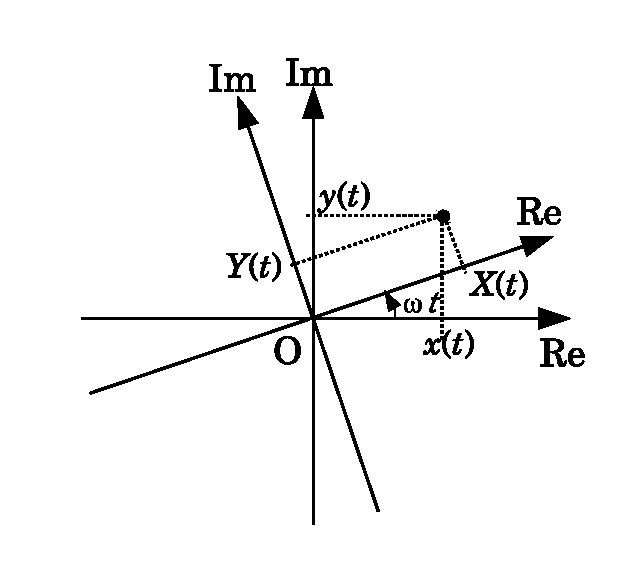
\includegraphics[width=6cm]{inert_circle.eps}
    \caption{慣性系$O$と, それに対して回転する座標系$O'$。複素平面で表現する。傾いてるのが座標系$O'$}\label{fig:inert_circle}
\end{figure}

座標系$O'$において, 質点の位置と質点にかかる力はそれぞれ, 
\begin{eqnarray}
{\bf R}(t)&=&(X(t), Y(t))\\
{\bf F}(t)&=&(F_X(t), F_Y(t))
\end{eqnarray}
とあらわされるとする。慣性系$O$について考えたときと同様に, 座標系$O'$でのベクトル${\bf R}(t)$, ${\bf F}(t)$
にそれぞれ対応する複素数$R(t)$, $F(t)$を考える。すなわち, 
\begin{eqnarray}
R(t)&=&X(t)+iY(t)\\
F(t)&=&F_X(t)+iF_Y(t)
\end{eqnarray}
とする。

座標系$O'$の座標軸は慣性系$O$の座標軸に対して$\omega\,t$だけ回転するから, $O$における座標成分
(つまり${\bf r}(t)$の成分)は$O'$における座標成分(つまり${\bf R}(t)$の成分)を
$\omega\,t$だけ回転したものになる。従って, 
\begin{eqnarray}
r(t)&=&R(t)e^{i\,\omega\,t}\label{eq:rRrotat}\\
f(t)&=&F(t)e^{i\,\omega\,t}\label{eq:fFrotat}
\end{eqnarray}
となる。

さて, \eref{eq:rRrotat}の両辺を$t$で微分すると, 
\begin{eqnarray}r'(t)=R'(t)e^{i\,\omega\,t}+i\,\omega R(t)e^{i\,\omega\,t}\end{eqnarray}
となる。もういちど両辺を$t$で微分すると, 
\begin{eqnarray}r''(t)=R''(t)e^{i\,\omega\,t}&+&2i\,\omega R'(t)e^{i\,\omega\,t}\nonumber\\
                                            &-&\omega^2 R(t)e^{i\,\omega\,t}\end{eqnarray}
となる。両辺に$m$をかけると, 
\begin{eqnarray}mr''(t)=mR''(t)e^{i\,\omega\,t}&+&2im\omega R'(t)e^{i\,\omega\,t}\nonumber\\
                                            &-&m\omega^2 R(t)e^{i\,\omega\,t}\end{eqnarray}
$f(t)=mr''(t)$に注意すると, 
\begin{eqnarray}f(t)=mR''(t)e^{i\,\omega\,t}&+&2im\omega R'(t)e^{i\,\omega\,t}\nonumber\\
                                            &-&m\omega^2 R(t)e^{i\,\omega\,t}\end{eqnarray}
となる。\eref{eq:fFrotat}に注意すると, 
\begin{eqnarray}F(t)e^{i\,\omega\,t}=mR''(t)e^{i\,\omega\,t}&+&2im\omega R'(t)e^{i\,\omega\,t}\nonumber\\
                                            &-&m\omega^2 R(t)e^{i\,\omega\,t}\end{eqnarray}
となる。両辺の全ての項に$e^{i\,\omega\,t}$が掛かっているのでこれを約分する(つまり
両辺に$e^{-i\,\omega\,t}$をかける)と, 
\begin{eqnarray}
F(t)=mR''(t)+2im\omega R'(t)-m\omega^2 R(t)
\end{eqnarray}
となる。右辺の第2項と第3項を左辺に移せば, 
\begin{eqnarray}
F(t)-2im\omega R'(t)+m\omega^2 R(t)=mR''(t)
\end{eqnarray}
となる。この式は, 座標系$O'$でも成り立つ「運動方程式に似たような式」である。ここで, 
\begin{eqnarray}
-2im\omega R'(t)+m\omega^2 R(t)\label{eq:rotinertf}
\end{eqnarray}
を慣性力として考えよう。\eref{eq:rotinertf}の最初の項$-2im\omega R'(t)$は, 
$R'(t)$, つまり座標系$O'$での速度に, $-i$がかかっている。複素平面で$-i$を
かけるということは, $y$軸から$x$軸に向かう向き(「慣性系$O$からみた座標系$O'$の回転の方向」の逆向き)
に90度回転することに相当する。つまりこの慣性力は, 
速度に対して直角にかかる。また, その大きさは速度と角速度$\omega$に比例する。このような慣性力を, 
\underline{コリオリ力}\index{こりおりりょく@コリオリ力}という。

\eref{eq:rotinertf}の2番目の項$m\omega^2 R(t)$は, $R(t)$, つまり座標系$O'$での位置と, 角速度$\omega$の2乗に, 
それぞれ比例し, $R(t)$と同じ向き(原点から離れる方向)にかかる。このような慣性力を, 
\underline{遠心力}\index{えんしんりょく@遠心力}という。
\vspace{0.2cm}

\begin{q}\label{q:inert_frame_rot_0}
慣性系$O$に対して一定の角速度$\omega$で回転する座標系$O'$において生じる慣性力を導出し, 
それぞれがどう呼ばれるかを述べよ。(上の議論を再現すればOK)。
\end{q}
\mv

\begin{q}\label{q:inert_frame_rot}
北極点上空を速さ$v$で飛ぶ, 質量$m$の飛行機を考える。地球の自転の角速度を$\omega$とする。
\begin{enumerate}
\item 飛行機にかかるコリオリ力の大きさを$m$, $\omega$, $v$で表せ。
\item 飛行機にかかるコリオリ力は重力の約何倍か? ただし$v=$1000\,km$\,$h$^{-1}$とする。
\item 飛行機はまっすぐ飛んだつもりでも, その軌跡はコリオリ力によって横方向にずれる。1時間の飛行によってどのくらい横にずれるか?
\end{enumerate}
\end{q}
\mv

\begin{q}\label{q:centrifuge}
回転半径15~cm, 単位時間あたりの回転数が4000~rpmの遠心分離器がある(rpmはrotation per minute, 
すなわち1分間あたりの回転数)。この遠心分離器で, 試料溶液中の懸濁物を沈降させようと思う。遠心分離器
なしで, 地上の重力にまかせて3.0日かかる沈降は, この遠心分離器を使うとどのくらいの時間に短縮できるか?
ただし沈降時の粒子にかかる抵抗力は沈降速度に比例するとする。
\end{q}
\mv

\begin{q}\label{q:IMU} 慣性計測装置(IMU)とは何かを述べ, その農業利用の
例を挙げ, その仕組みをわかりやすく自分の言葉で説明せよ。\end{q}\mv

%\begin{q}\label{q:plane} 雲や霧の中で視界のほとんど無い状態で飛行機が落下を始めると, 
%操縦士はどちらが上なのかわからなくなってしまうらしい。なぜだろう?\end{q}\mv

\begin{q}\label{q:typhoon} 台風について考える。
\begin{enumerate}
\item 北半球の台風の渦は, どのような向きに巻いているか? それはなぜか?
\item 北半球では, 台風の進行方向を向いて右側(多くの場合は東側)は左側より風が強いことが多い。なぜか?
\item 1991年の台風19号は, 九州に大規模な倒木被害をもたらし, 青森では収穫前のリンゴの多くが落果した。このような大きな被害をもたらした背景を, この台風の進路や勢力で説明せよ。
\item 台風は熱帯地方で発生するが, 奇妙なことに, 熱帯のど真ん中である赤道付近では台風は発生しない。なぜか?
\end{enumerate}
\end{q}\mv

\begin{exq} 国際宇宙ステーションの中が「無重力」なのはなぜなのか, 説明せよ。\end{exq}\mv

\begin{exq} つくばエキスプレスのつくば行き快速電車は, つくば駅の1.0~km手前から減速し, つくば駅で停車する。
減速直前の列車の速度を$v=$100~km/hとする。減速中の車内で列車後尾に向かって歩く人は, まるで坂道を登って
いるかのような負荷を感じる。それは傾斜何度程度の坂道に相当するか? 列車は加速度$a$の等加速度直線運動
をするとみなしてよい。\end{exq}

\hv


\section{解答}

%日本のH2A宇宙ロケットは, 打ち上げ後, 約100秒間で高度約50kmに到達する。
\noindent{\textbf{答}}\ref{q:inert_frame_H2}
\begin{enumerate}
\item 一定加速度を$a$とする。打ち上げの瞬間を時刻0とする。時刻$t$までの飛距離$x$は$x=at^2/2$。従って, 
\begin{eqnarray*}
a=\frac{2x}{t^2}
\end{eqnarray*}
これに$t=100\,$s, $x=50000\,$mを代入すると, $a=10\,$m s$^{-2}$。注意: 実際はロケットの運動は等加速度運動ではない。その理由のひとつとして, 燃料消費に伴って, 質量が刻々と減っていくことがある。
\item 質量を$m$とすると, 慣性力は$ma$。一方, 重力は$mg$。両者を比較すると, $a=10$~m~s$^{-2}$と$g$はほとんど同じなので, 慣性力は(地上付近での)重力にほぼ等しい。ただし, この慣性力は加速方向(上向き)とは逆方向(下向き)にかかるので, 重力と慣性力の合力は, 重力の約2倍(下向き)となる。
\end{enumerate}
\vspace{0.2cm}

\noindent{\textbf{答}}\ref{q:inert_frame_rot_0} 略。\mv

% 北極点上空を早さ$v$で飛ぶ, 質量$m$の飛行機を考える。地球の自転の角速度を$\omega$とする。
\noindent{\textbf{答}}\ref{q:inert_frame_rot}
\begin{enumerate}
\item \eref{eq:rotinertf}の第1項より, 飛行機にかかるコリオリ力の大きさは$2m\omega v$。
\item 地球の自転の周期を$T$とすると, 角速度は
\begin{eqnarray*}\omega=\frac{2\pi}{T}=\frac{2\times3.14}{60\times60\times24\text{ s}}=7.27\times10^{-5}\text{ s}^{-1}
\end{eqnarray*}
一方, $v=$1000 km h$^{-1}$を換算すると, \\$v=278$~m~s$^{-1}$。従って, 
\begin{eqnarray*}
2\omega v&=&2\times7.27\times10^{-5}\text{ s}^{-1}\times278\text{ m s}^{-1}\\
          &=&0.0404\text{ m s}^{-2}
\end{eqnarray*}
これは重力加速度の約0.004倍。
\item 本来は円運動になるはずだが, 横方向の等加速度運動として近似すると(加速度$a$は(2)で求めた値), 
時間$t=3600$ sの間に横方向の移動距離は$at^2/2$になるから, 
\begin{eqnarray*}
\frac{0.0404\text{ m s}^{-2}\times (3600 \text{ s})^2}{2}=2.6\times10^5\,\,\text{m}
\end{eqnarray*}
すなわち, 約260 km。
\end{enumerate}

\noindent{\textbf{答}}\ref{q:centrifuge} 略。\mv

\noindent{\textbf{答}}\ref{q:IMU} 略。\mv

\noindent{\textbf{答}}\ref{q:typhoon} 略。\mv

